\section{Extended Results}

\subsection{Extended Results: Scaling Laws}
\label{app:scaling-laws}

\begin{table}
\centering            % always nice to centre floats
\scriptsize         % <── was \small; try \footnotesize or \scriptsize
\setlength{\tabcolsep}{3pt}
% \begin{adjustbox}{width=\textwidth}
\caption{\textbf{A summary of the monolingual scaling laws for each language}
The columns are: the language, the language family, the language script, its number of unique tokens $|D|$ in \madlad{} (with the percentage of unique tokens as compared to English), and the derived scaling law. 
}
\begin{tabular}{l|lll|l}
\toprule
\textsc{Language} & \textsc{Family} & \textsc{Script} & \textsc{$|D|$ (\% EN)} &
\textsc{Scaling Law} \\
\midrule
\multicolumn{5}{c}{\textsc{\emph{Monolingual Vocabulary, Monolingual Training}}} \\
\midrule
      
English & Indo-european & Latin & 2.8T (100.0\%) & $\,0.67\;+\;\frac{e^{6.18}}{N^{0.41}}\;+\;\frac{e^{8.25}}{D^{0.41}}\,$ \\[2mm]
French & Indo-european & Latin & 363B (13.01\%) & $\,0.76\;+\;\frac{e^{10.11}}{N^{0.64}}\;+\;\frac{e^{13.24}}{D^{0.64}}\,$ \\[2mm]
Russian & Indo-european & Cyrillic & 705B (25.26\%) & $\,0.82\;+\;\frac{e^{10.07}}{N^{0.63}}\;+\;\frac{e^{13.28}}{D^{0.63}}\,$ \\[2mm]
Chinese & Sino-tibetan & Hans & 125B (4.48\%) & $\,1.08\;+\;\frac{e^{8.20}}{N^{0.46}}\;+\;\frac{e^{10.37}}{D^{0.46}}\,$ \\[2mm]
Hindi & Indo-european & Devanagari & 7.9B (0.28\%) & $\,0.52\;+\;\frac{e^{6.03}}{N^{0.39}}\;+\;\frac{e^{8.03}}{D^{0.39}}\,$ \\[2mm]
Swahili & Niger-congo: atlantic congo & Latin & 770M (0.03\%) & $\,0.00\;+\;\frac{e^{4.13}}{N^{0.26}}\;+\;\frac{e^{5.51}}{D^{0.26}}\,$ \\[2mm]


\midrule
\multicolumn{5}{c}{\textsc{\emph{Multilingual Vocabulary, Monolingual Training}}} \\
\midrule

English & Indo-european & Latin & 2.8T (100.0\%) & $\,0.83\;+\;\frac{e^{9.91}}{N^{0.63}}\;+\;\frac{e^{13.06}}{D^{0.63}}\,$ \\[2mm]
French & Indo-european & Latin & 363B (13.01\%) & $\,0.66\;+\;\frac{e^{7.12}}{N^{0.45}}\;+\;\frac{e^{8.94}}{D^{0.45}}\,$ \\[2mm]
Russian & Indo-european & Cyrillic & 705B (25.26\%) & $\,0.76\;+\;\frac{e^{7.97}}{N^{0.49}}\;+\;\frac{e^{9.91}}{D^{0.49}}\,$ \\[2mm]
Chinese & Sino-tibetan & Hans & 125B (4.48\%) & $\,1.18\;+\;\frac{e^{8.87}}{N^{0.49}}\;+\;\frac{e^{10.90}}{D^{0.49}}\,$ \\[2mm]
Hindi & Indo-european & Devanagari & 7.9B (0.28\%) & $\,0.63\;+\;\frac{e^{6.99}}{N^{0.43}}\;+\;\frac{e^{8.69}}{D^{0.43}}\,$ \\[2mm]
Swahili & Niger-congo: atlantic congo & Latin & 770M (0.03\%) & $\,0.00\;+\;\frac{e^{4.99}}{N^{0.30}}\;+\;\frac{e^{6.43}}{D^{0.30}}\,$ \\[2mm]

\midrule
\multicolumn{5}{c}{\textsc{\emph{Multilingual Vocabulary, Unimax Training}}} \\
\midrule

English & Indo-european & Latin & 2.8T (100.0\%) & $\,0.00\;+\;\frac{e^{3.03}}{N^{0.16}}\;+\;\frac{e^{3.15}}{D^{0.16}}\,$ \\[2mm]
French & Indo-european & Latin & 363B (13.01\%) & $\,0.00\;+\;\frac{e^{3.63}}{N^{0.19}}\;+\;\frac{e^{3.94}}{D^{0.19}}\,$ \\[2mm]
Russian & Indo-european & Cyrillic & 705B (25.26\%) & $\,0.00\;+\;\frac{e^{3.90}}{N^{0.20}}\;+\;\frac{e^{4.28}}{D^{0.20}}\,$ \\[2mm]
Chinese & Sino-tibetan & Hans & 125B (4.48\%) & $\,0.39\;+\;\frac{e^{4.58}}{N^{0.21}}\;+\;\frac{e^{5.47}}{D^{0.21}}\,$ \\[2mm]
Hindi & Indo-european & Devanagari & 7.9B (0.28\%) & $\,0.00\;+\;\frac{e^{3.46}}{N^{0.18}}\;+\;\frac{e^{3.89}}{D^{0.18}}\,$ \\[2mm]
Swahili & Niger-congo: atlantic congo & Latin & 770M (0.03\%) & $\,0.00\;+\;\frac{e^{3.52}}{N^{0.18}}\;+\;\frac{e^{3.74}}{D^{0.18}}\,$ \\[2mm]

\bottomrule
\end{tabular}
% \end{adjustbox}
% \vspace{1mm}
\label{tab:mono-scaling-laws}
% \vspace{-5mm}
\end{table}

In \Cref{tab:mono-scaling-laws} we illustrate the fitted scaling laws for each language.
Specifically, we show the scaling law parameters for each language when trained with a monolingual vocabulary on monolingual data, when trained with a multilingual vocabulary on monolingual data, and when trained with a multilingual vocabulary on the \unimax{} multilingual mixture.
These results match up with those presented in \Cref{fig:monolingual-scaling}.

\subsection{Extended Results: Language Transfer}
\label{app:lang-transfer}

\textbf{Research Question:} \emph{How does language transfer change with larger models, or when you train for longer?}

We further investigated how language transfer evolves with training data (D) and model size (N) in \Cref{fig:language-transfer-nd}. Our analysis of transfer scores over the course of training reveals that transfer dynamics are established early. The performance gap between synergistic pairs (e.g., es $\rightarrow$ pt) and interfering pairs (e.g., en $\rightarrow$ zh) appears within the initial stages of training and remains largely consistent, suggesting that the fundamental compatibility of languages is not significantly altered by longer training. However, the impact of model scale is more pronounced. As illustrated in \Cref{fig:language-transfer-nd}, we observe a clear trend in which larger models are more effective in facilitating cross-lingual transfer. For synergistic pairs, the positive transfer score increases modestly with model capacity. More importantly, for challenging pairs that exhibit interference in smaller models, larger models are significantly better at mitigating this negative effect, bringing the score closer to zero.  This is similar to what has been observed while training larger and larger foundation models \citep{team2024gemini}. Given that transfer dynamics change at scale, it is an important factor to consider when designing multilingual foundation models that are performant for all languages being trained on. 

% For instance, \sneha{get example language pairs}.
% \sneha{Feels a lil filler: This suggests that increased model capacity is crucial for overcoming the "curse of multilinguality," as it allows the model to learn shared, beneficial representations in distinct parameter subspaces rather than suffering from catastrophic interference.}


\begin{figure*}
    \centering
    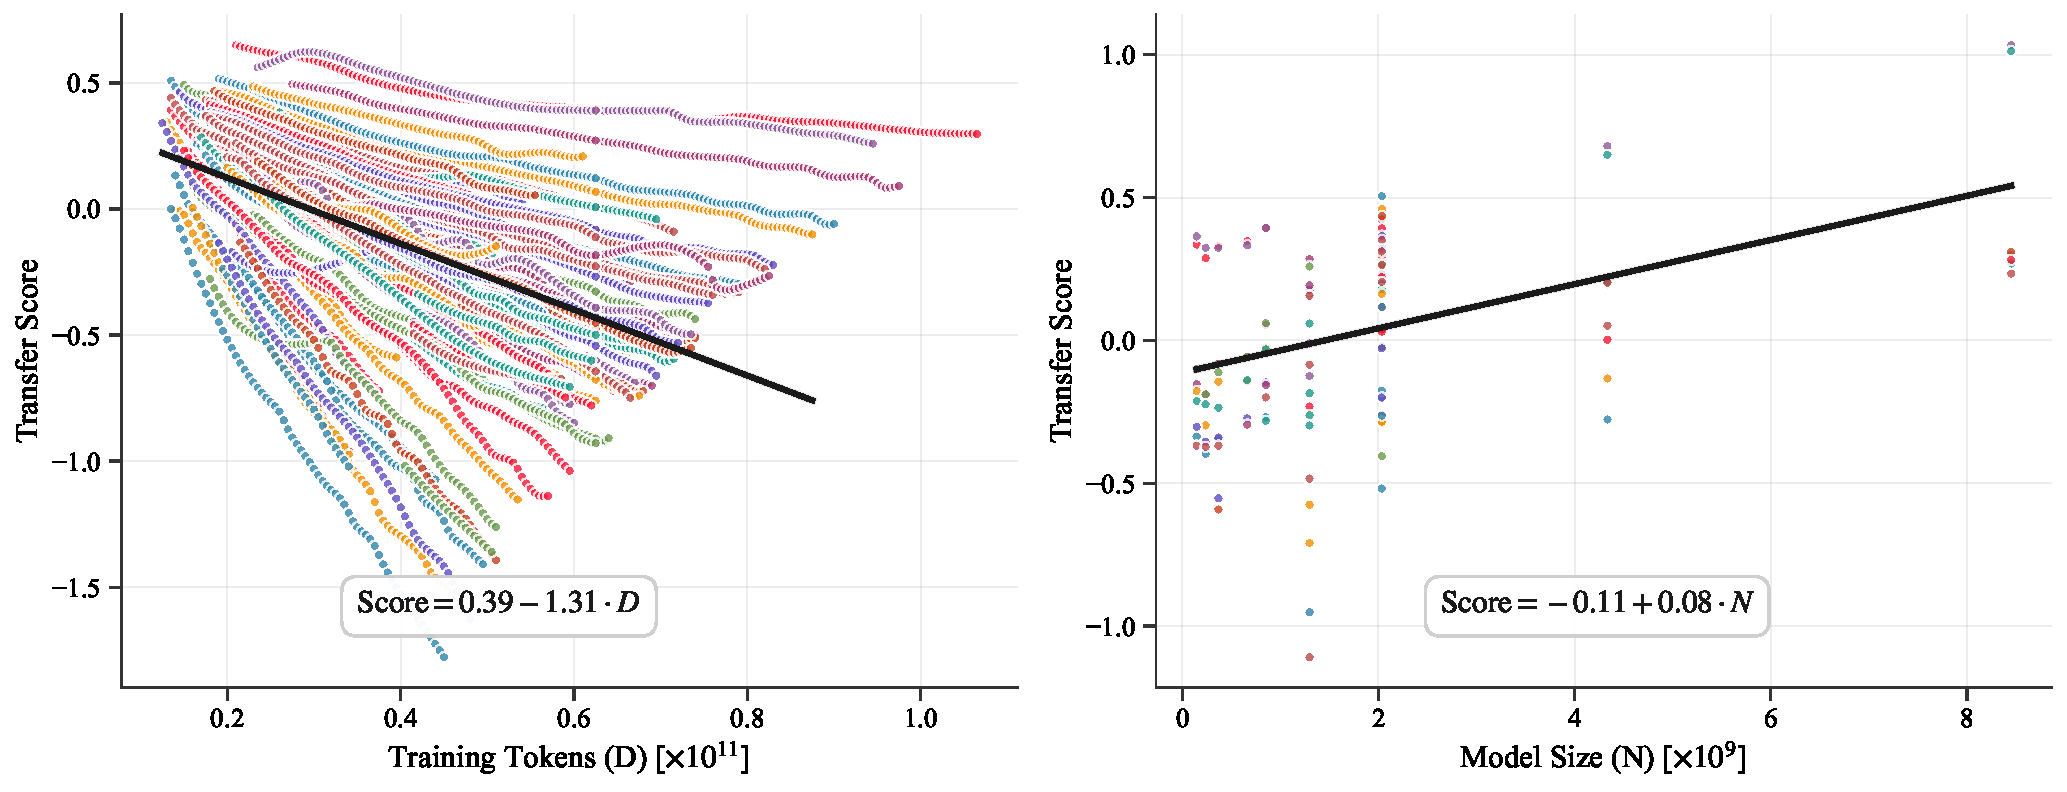
\includegraphics[width=\textwidth]{figures/language-transfer/langtransfer_dn_score_publication.pdf}
    \caption{
    \textbf{Left:} X-axis is training tokens (D), Y-axis is language-transfer score.
    \textbf{Right:} X-axis is model size (N), Y-axis is language-transfer score.}
    \label{fig:language-transfer-nd}
    \vspace{-4mm}
% \begin{figure*}[t]
%   \centering
%   %----------------------- Left panel ----------------------
%   \begin{subfigure}[t]{.5\textwidth}
%     \includegraphics[width=\linewidth]{figures/language-transfer/langtransfer_d_score.pdf}
%     \caption{X-axis is training tokens (D), Y-axis is language-transfer score.}
%     \label{fig:language-transfer-d}
%   \end{subfigure}%
%   % ← the percent sign above kills the inter-box whitespace
%   %---------------------- Right panel ----------------------
%   \begin{subfigure}[t]{.5\textwidth}
%     \includegraphics[width=\linewidth]{figures/language-transfer/langtransfer_n_score.pdf}
%     \caption{X-axis is model size (N), Y-axis is language-transfer score.}
%     \label{fig:language-transfer-n}
%   \end{subfigure}

  % \caption{\TODO{FIX FIGURE: (0) Remove titles. Add better x- and y-axis labels, and increase the font size of the ticks and labels so they are more visible. Make each figure larger, and position them so when they are side-by-side there is less whitespace between them (a tighter display). (1) Add lines connecting relevant points in the rightside figure, like in the leftside one (maybe, see how it looks). (2) Get better lines of best fit and have them annotated in a box, so we know the formula and gradient of each just by looking at the figure. (3) I don't think I like the style of having each figure in a black box. Let's just have the x and y axis visible.} \niklas{Similar to heatmap, maybe worth pointing to explanation of the transfer score so readers can reason more easily about what y=0.5 means} \sneha{nice - could we have a legend for this so we can improve the story in the text}}
\end{figure*}


\begin{figure*}
    \centering
    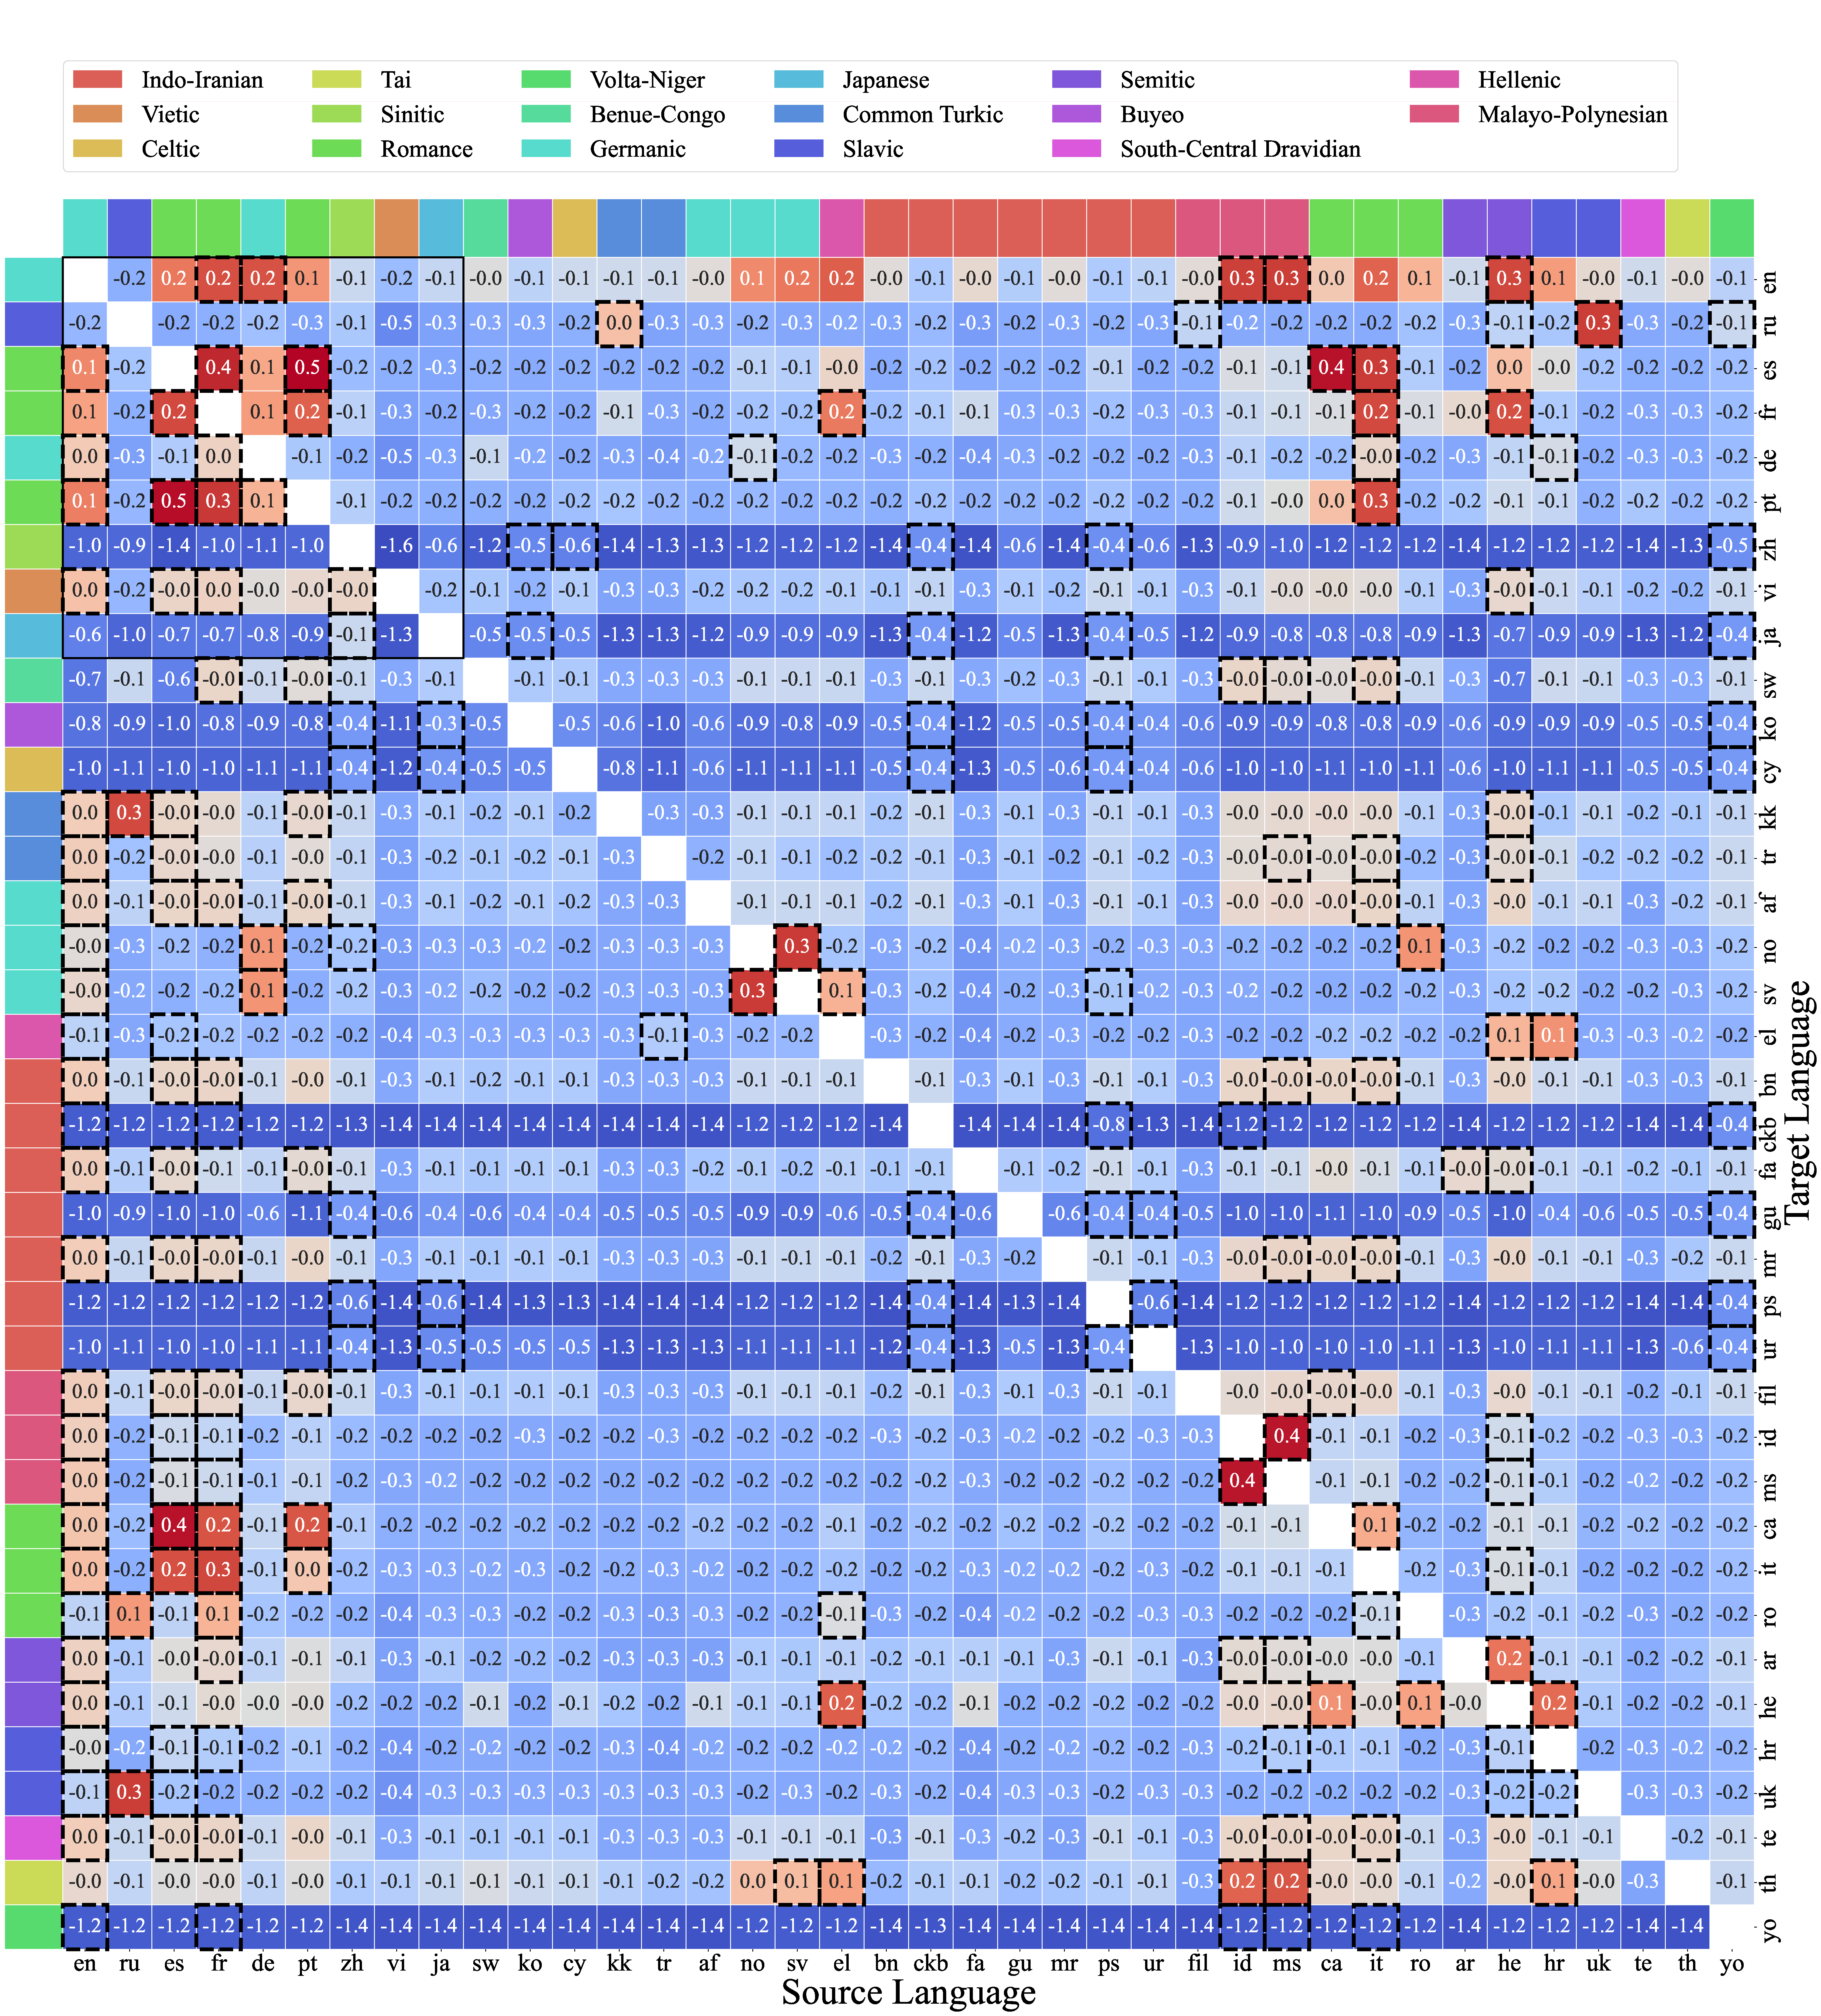
\includegraphics[width=0.9\textwidth]{figures/language-transfer/multilingual_heatmap_v1.pdf}
    \caption{The language transfer scores measure the benefit to the target language of (co-)training with the source language. We bold the top-5 source languages for each target language. The top left 9x9 are the Bilingual Transfer Score computed directly, whereas the rest are estimated from the Finetuning Adaptation Score. While English is the best source language for many of  of languages, we find language similarity is highly predictive of these scores.  \label{fig:language-transfer-heatmap-full}}
\end{figure*}
